\PassOptionsToPackage{enable-debug,check-declarations}{expl3}
\RequirePackage{pdfmanagement-testphase}
\DeclareDocumentMetadata {  }
\ExplSyntaxOn
\pdfmanagement_add:nnn{Catalog}{Lang}{(enUS)}
\ExplSyntaxOff

% xmp metadata for pdf
% Originally used \usepackage[a-2a]{pdfx}
% \usepackage{hyperxmp} replaced it
% \RequirePackage{pdfmanagement-testphase} replaced it

\documentclass[11pt,
  english,
  a4paper,
]{article}
\usepackage{sa4ss}
\usepackage{amsmath,amssymb,array}
\usepackage{booktabs}

% From tagged-template.latex
\usepackage{lmodern}
\usepackage{ifxetex,ifluatex}
\ifnum 0\ifxetex 1\fi\ifluatex 1\fi=0 % if pdftex
  \usepackage[T1]{fontenc}
  \usepackage[utf8]{inputenc}
  \usepackage{textcomp} % provide euro and other symbols
\else % if luatex or xetex
  \usepackage{unicode-math}
  \defaultfontfeatures{Scale=MatchLowercase}
  \defaultfontfeatures[\rmfamily]{Ligatures=TeX,Scale=1}
\fi

% Use upquote if available, for straight quotes in verbatim environments
\IfFileExists{upquote.sty}{\usepackage{upquote}}{}
\IfFileExists{microtype.sty}{% use microtype if available
  \usepackage[]{microtype}
  \UseMicrotypeSet[protrusion]{basicmath} % disable protrusion for tt fonts
}{}
\makeatletter
\@ifundefined{KOMAClassName}{% if non-KOMA class
  \IfFileExists{parskip.sty}{%
    \usepackage{parskip}
  }{% else
    \setlength{\parindent}{0pt}
    \setlength{\parskip}{6pt plus 2pt minus 1pt}}
}{% if KOMA class
  \KOMAoptions{parskip=half}}
\makeatother
\usepackage{xcolor}
\IfFileExists{xurl.sty}{\usepackage{xurl}}{} % add URL line breaks if available
\hypersetup{
  pdftitle={The status of Vermilion Rockfish (Sebastes miniatus) and Sunset Rockfish (Sebastes crocotulus) in U.S. waters off the coast of California north of Pt. Conception in 2021},
  pdflang={en},
  hidelinks,
  pdfcreator={LaTeX via pandoc}}
\urlstyle{same} % disable monospaced font for URLs
\usepackage{longtable}
% Correct order of tables after \paragraph or \subparagraph
\usepackage{etoolbox}
\makeatletter
\patchcmd\longtable{\par}{\if@noskipsec\mbox{}\fi\par}{}{}
\makeatother
% Allow footnotes in longtable head/foot
\IfFileExists{footnotehyper.sty}{\usepackage{footnotehyper}}{\usepackage{footnote}}
\makesavenoteenv{longtable}
\usepackage{graphicx}
\makeatletter
\def\maxwidth{\ifdim\Gin@nat@width>\linewidth\linewidth\else\Gin@nat@width\fi}
\def\maxheight{\ifdim\Gin@nat@height>\textheight\textheight\else\Gin@nat@height\fi}
\makeatother
% Scale images if necessary, so that they will not overflow the page
% margins by default, and it is still possible to overwrite the defaults
% using explicit options in \includegraphics[width, height, ...]{}
\setkeys{Gin}{width=\maxwidth,height=\maxheight,keepaspectratio}
% Set default figure placement to htbp
\makeatletter
\def\fps@figure{htbp}
\makeatother
\setlength{\emergencystretch}{3em} % prevent overfull lines
\providecommand{\tightlist}{%
  \setlength{\itemsep}{0pt}\setlength{\parskip}{0pt}}
\setcounter{secnumdepth}{5}
\usepackage{booktabs}
\usepackage{longtable}
\usepackage{array}
\usepackage{multirow}
\usepackage{wrapfig}
\usepackage{float}
\usepackage{colortbl}
\usepackage{pdflscape}
\usepackage{tabu}
\usepackage{threeparttable}
\usepackage[normalem]{ulem}
\usepackage{makecell}
\usepackage{xcolor}
\usepackage{placeins}
\ifxetex
  % Load polyglossia as late as possible: uses bidi with RTL langages (e.g. Hebrew, Arabic)
  \usepackage{polyglossia}
  \setmainlanguage[]{english}
\else
  \usepackage[shorthands=off,main=english]{babel}
\fi

%Define cslreferences environment, required by pandoc 2.8
%https://github.com/rstudio/rmarkdown/issues/1649
\newlength{\csllabelwidth}
\setlength{\csllabelwidth}{3em}
\newlength{\cslhangindent}
\setlength{\cslhangindent}{1.5em}
% for Pandoc 2.8 to 2.10.1
\newenvironment{cslreferences}%
  {}%
  {\par}
% For Pandoc 2.11+
\newenvironment{CSLReferences}[2] % #1 hanging-ident, #2 entry spacing
 {% don't indent paragraphs
  \setlength{\parindent}{0pt}
  % turn on hanging indent if param 1 is 1
  \ifodd #1 \everypar{\setlength{\hangindent}{\cslhangindent}}\ignorespaces\fi
  % set entry spacing
  \ifnum #2 > 0
  \setlength{\parskip}{#2\baselineskip}
  \fi
 }%
 {}
\usepackage{calc}  % for \widthof, \maxof in minipage
\newcommand{\CSLBlock}[1]{#1\hfill\break}
\newcommand{\CSLLeftMargin}[1]{\parbox[t]{\csllabelwidth}{#1}}
\newcommand{\CSLRightInline}[1]{\parbox[t]{\linewidth - \csllabelwidth}{#1}\break}
\newcommand{\CSLIndent}[1]{\hspace{\cslhangindent}#1}


\providecommand{\tightlist}{%
  \setlength{\itemsep}{0pt}\setlength{\parskip}{0pt}}

\usepackage{booktabs}
\usepackage{longtable}
\usepackage{array}
\usepackage{multirow}
\usepackage{wrapfig}
\usepackage{float}
\usepackage{colortbl}
\usepackage{pdflscape}
\usepackage{tabu}
\usepackage{threeparttable}
\usepackage[normalem]{ulem}
\usepackage{makecell}
\usepackage{xcolor}
\usepackage{placeins}
\date{}
\newcommand{\trTitle}{The status of Vermilion Rockfish (\emph{Sebastes miniatus}) and Sunset Rockfish (\emph{Sebastes crocotulus}) in U.S. waters off the coast of California north of Pt. Conception in 2021}
\newcommand{\trYear}{2021}
\newcommand{\trMonth}{June}
\newcommand{\trAuthsLong}{truetruetruetrue}
\newcommand{\trAuthsBack}{Monk, M.H., E.J. Dick, J.C. Field, E.M. Saas}
\newcommand{\trCitation}{
\begin{hangparas}{1em}{1}
\trAuthsBack{}. \trYear{}. \trTitle{}. Pacific Fisheries Management Council, Portland, Oregon. \pageref{LastPage}{}\,p.
\end{hangparas}}

\AtBeginDocument{\tagstructbegin{tag=Document}}
\AtEndDocument{\tagstructend}
\pretocmd{\maketitle}{\tagstructbegin{tag=H1}\tagmcbegin{tag=H1}}{}{}
\apptocmd{\maketitle}{\tagmcend\tagstructend}{}{}

\begin{document}

%%%%% Frontmatter %%%%%

% Footnote symbols in front matter
\renewcommand*{\thefootnote}{\fnsymbol{footnote}}

\small
\thispagestyle{empty}
\pagenumbering{roman}
\noindent
\begin{center}
\title{The status of Vermilion Rockfish (\emph{Sebastes miniatus}) and Sunset Rockfish (\emph{Sebastes crocotulus}) in U.S. waters off the coast of California north of Pt. Conception in 2021}
% \textnormal{\MakeTextUppercase{\trTitle{}}}
\vspace{1.5cm}
{\Large\textbf\newline{The status of Vermilion Rockfish (\emph{Sebastes miniatus}) and Sunset Rockfish (\emph{Sebastes crocotulus}) in U.S. waters off the coast of California north of Pt. Conception in 2021}}
\vfill
by\\
Melissa H. Monk\textsuperscript{1}\\
E. J. Dick\textsuperscript{1}\\
John C. Field\textsuperscript{1}\\
Emma M. Saas\textsuperscript{1}\vfill
\textsuperscript{1}Southwest Fisheries Science Center, U.S. Department of Commerce, National Oceanic and Atmospheric Administration, National Marine Fisheries Service, 110 McAllister Way, Santa Cruz, California 95060\vfill
\trMonth{} \trYear{}
\end{center}
\clearpage

% Fourth page: Colophon
\thispagestyle{empty}
\vspace*{\fill}
\begin{center}
\copyright{} Pacific Fisheries Management Council, \trYear{}\\
\end{center}
\par
\bigskip
\noindent
Correct citation for this publication:
\bigskip
\par
\trCitation{}
\clearpage

% Add TOC to pdf bookmarks (clickable pdf)
\pdfbookmark[1]{\contentsname}{toc}

% Table of contents page, lists of figures and tables
\tableofcontents\clearpage
\label{TRlastRoman}
\clearpage

% Table of contents
\newpage
\thispagestyle{empty} % to remove page number

% Settings for the main document
\pagenumbering{arabic}  % Regular page numbers
\pagestyle{plain}  % No page number on first page of main document, use 'empty'
\renewcommand*{\thefootnote}{\arabic{footnote}}  % Back to numeric footnotes
\setcounter{footnote}{0}  % And start at 1
\renewcommand{\headrulewidth}{0.5pt}
\renewcommand{\footrulewidth}{0.5pt}
%\pagestyle{fancy}\fancyhead[c]{Draft: Do not cite or circulate}

\newcommand{\lt}{\ensuremath <}
\newcommand{\gt}{\ensuremath >}

\pagebreak
\pagenumbering{roman}
\setcounter{page}{1}

\renewcommand{\thetable}{\roman{table}}
\renewcommand{\thefigure}{\roman{figure}}

\setlength\parskip{0.5em plus 0.1em minus 0.2em}

\tagstructbegin{tag=H1}\tagmcbegin{tag=H1}

\hypertarget{executive-summary}{%
\section*{Executive Summary}\label{executive-summary}}
\addcontentsline{toc}{section}{Executive Summary}

\leavevmode\tagmcend\tagstructend

To be completed after the STAR panel.

\tagstructbegin{tag=H2}\tagmcbegin{tag=H2}

\hypertarget{stock}{%
\subsection*{Stock}\label{stock}}
\addcontentsline{toc}{subsection}{Stock}

\leavevmode\tagmcend\tagstructend

This assessment reports the status of the vermlion rockfish (\emph{Sebastes miniatus}) and sunset rockfish (\emph{Sebastes crocotulus}) complex (referred to as vermilion throughout), resource in U.S. waters off the coast of California north of Point Conception ({\tagstructbegin{tag=Formula}\tagmcbegin{tag=Formula}\(34^\circ 27^\prime\)\leavevmode\tagmcend\tagstructend} N. latitude) using data through 2020.

\tagstructbegin{tag=H2}\tagmcbegin{tag=H2}

\hypertarget{landings}{%
\subsection*{Landings}\label{landings}}
\addcontentsline{toc}{subsection}{Landings}

\leavevmode\tagmcend\tagstructend

Replace text.

\tagstructbegin{tag=H2}\tagmcbegin{tag=H2}

\hypertarget{data-and-assessment}{%
\subsection*{Data and Assessment}\label{data-and-assessment}}
\addcontentsline{toc}{subsection}{Data and Assessment}

\leavevmode\tagmcend\tagstructend

Replace text.

\tagstructbegin{tag=H2}\tagmcbegin{tag=H2}

\hypertarget{stock-biomass}{%
\subsection*{Stock Biomass}\label{stock-biomass}}
\addcontentsline{toc}{subsection}{Stock Biomass}

\leavevmode\tagmcend\tagstructend

Replace text.

\tagstructbegin{tag=H2}\tagmcbegin{tag=H2}

\hypertarget{recruitment}{%
\subsection*{Recruitment}\label{recruitment}}
\addcontentsline{toc}{subsection}{Recruitment}

\leavevmode\tagmcend\tagstructend

Replace text.

\tagstructbegin{tag=H2}\tagmcbegin{tag=H2}

\hypertarget{exploitation-status}{%
\subsection*{Exploitation Status}\label{exploitation-status}}
\addcontentsline{toc}{subsection}{Exploitation Status}

\leavevmode\tagmcend\tagstructend

Replace text.

\tagstructbegin{tag=H2}\tagmcbegin{tag=H2}

\hypertarget{reference-points}{%
\subsection*{Reference Points}\label{reference-points}}
\addcontentsline{toc}{subsection}{Reference Points}

\leavevmode\tagmcend\tagstructend

Replace text.

\tagstructbegin{tag=H2}\tagmcbegin{tag=H2}

\hypertarget{management-performance}{%
\subsection*{Management Performance}\label{management-performance}}
\addcontentsline{toc}{subsection}{Management Performance}

\leavevmode\tagmcend\tagstructend

Replace text.

\tagstructbegin{tag=H2}\tagmcbegin{tag=H2}

\hypertarget{unresolved-problems-and-major-uncertainties}{%
\subsection*{Unresolved Problems and Major Uncertainties}\label{unresolved-problems-and-major-uncertainties}}
\addcontentsline{toc}{subsection}{Unresolved Problems and Major Uncertainties}

\leavevmode\tagmcend\tagstructend

Replace text.

\tagstructbegin{tag=H2}\tagmcbegin{tag=H2}

\hypertarget{decision-table}{%
\subsection*{Decision Table}\label{decision-table}}
\addcontentsline{toc}{subsection}{Decision Table}

\leavevmode\tagmcend\tagstructend

Replace text.

\tagstructbegin{tag=H2}\tagmcbegin{tag=H2}

\hypertarget{research-and-data-needs}{%
\subsection*{Research and Data Needs}\label{research-and-data-needs}}
\addcontentsline{toc}{subsection}{Research and Data Needs}

\leavevmode\tagmcend\tagstructend

Replace text.

\pagebreak
\setlength{\parskip}{5mm plus1mm minus1mm}
\pagenumbering{arabic}
\setcounter{page}{1}
\renewcommand{\thefigure}{\arabic{figure}}
\renewcommand{\thetable}{\arabic{table}}
\setcounter{table}{0}
\setcounter{figure}{0}

\tagstructbegin{tag=H1}\tagmcbegin{tag=H1}

\hypertarget{introduction}{%
\section{Introduction}\label{introduction}}

\leavevmode\tagmcend\tagstructend

\tagstructbegin{tag=H2}\tagmcbegin{tag=H2}

\hypertarget{basic-information}{%
\subsection{Basic Information}\label{basic-information}}

\leavevmode\tagmcend\tagstructend

This assessment reports the status of the Vermilion Rockfish (\emph{Sebastes miniatus}) and Sunset Rockfish (\emph{Sebastes crocotulus}) in U.S. waters off the coast of California south of Pt. Conception through 2020.

\#\#Basic Information and Life History

\emph{Population Structure and Complex Assessment Considerations}

Provided by John Harms (NWFSC)

A group of researchers from the NWFSC and SWFSC is collaborating on a project to genotype tissue specimens collected from the vermilion and sunset rockfish cryptic pair captured during the West Coast Groundfish Bottom Trawl Survey and the Southern CA Shelf Rockfish Hook and Line Survey for the years 2004 - 2019. Funding for this project was obtained through the Saltonstall-Kennedy program for FY 2020 through a proposal led by representatives from Pacific States Marine Fisheries Commission and the commercial passenger fishing vessel industry in southern California.

After combining with specimens obtained through other collection efforts along the West Coast, approximately 25,000 tissue specimens will be analyzed. Some earlier efforts to separate this cryptic pair to species used mitochondrial DNA (mtDNA) markers. However, due to a one-way mitochondrial introgression from the vermilion genome into the sunset genome, a portion of the sunset rockfish population contains mitochondrial DNA sequences consistent with vermilion rockfish resulting in incorrect species assignments for these introgressed individuals during the prior research project. The current research has identified a robust suite of genetic markers within the nuclear genomes of the two species that definitively separates vermilion and sunset rockfish (including introgressed sunset rockfish), canary rockfish, first generation vermilion-sunset hybrids, and identifies emerging patterns of intraspecific stock structure within the two sister species.

Once the collected specimens have been genotyped, any species-specific differences in spatial and depth distribution, size composition, weight-length relationships, and other biological characteristics will be identified. Using previously collected otoliths and ovaries, the demographics of the two species including age and growth and reproductive biology parameters such as length and age at 50\% maturity and the prevalence of skip spawning will be explored and compared. These new genotyping results will be combined with data from the prior mtDNA work to evaluate whether introgressed sunset rockfish represent a biologically intermediate subform of the species complex. The effort also proposes to develop and test the efficacy of models to predict the relative proportion of the two species based upon explanatory variables including latitude, depth, species of co-occurrence, oceanographic parameters, habitat descriptors and/or other information. The anticipated completion of the genotyping of all specimens is approximately December 2021 with provision of final results by the end of FY 2022.

This research is aimed at providing information to support the successful stock assessment of this commercially and recreationally valuable cryptic species pair and is responsive to any data gaps identified by the assessment community. If successful, this research, conducted in close communication with stock assessors, may also assist the PFMC in establishing best practices for the assessment and management of cryptic species complexes. Though this project will only focus on nominal vermilion rockfish specimens collected through the 2019 survey field season, it may be advisable that tissue specimens collected aboard fishery-independent surveys as well as through fishery-dependent programs continue to be genotyped on an ongoing basis to support continued and timely monitoring of this economically and ecologically important species complex.

\tagstructbegin{tag=H2}\tagmcbegin{tag=H2}

\hypertarget{early-life-history}{%
\subsection{Early Life History}\label{early-life-history}}

\leavevmode\tagmcend\tagstructend

\#\#Map

\#\#Ecosystem Considerations

\tagstructbegin{tag=H2}\tagmcbegin{tag=H2}

\hypertarget{historical-and-current-fishery-information}{%
\subsection{Historical and Current Fishery Information}\label{historical-and-current-fishery-information}}

\leavevmode\tagmcend\tagstructend

Replace text.

\tagstructbegin{tag=H2}\tagmcbegin{tag=H2}

\hypertarget{summary-of-management-history-and-performance}{%
\subsection{Summary of Management History and Performance}\label{summary-of-management-history-and-performance}}

\leavevmode\tagmcend\tagstructend

Replace text.

\#\#Management Performance

\tagstructbegin{tag=H2}\tagmcbegin{tag=H2}

\hypertarget{foreign-fisheries}{%
\subsection{Foreign Fisheries}\label{foreign-fisheries}}

\leavevmode\tagmcend\tagstructend

Replace text.

\tagstructbegin{tag=H1}\tagmcbegin{tag=H1}

\hypertarget{data}{%
\section{Data}\label{data}}

\leavevmode\tagmcend\tagstructend

A description of each data source is provided below (Figure).

\tagstructbegin{tag=H2}\tagmcbegin{tag=H2}

\hypertarget{biological-data}{%
\subsection{Biological Data}\label{biological-data}}

\leavevmode\tagmcend\tagstructend

\tagstructbegin{tag=H3}\tagmcbegin{tag=H3}

\hypertarget{length-and-age-compositions}{%
\subsubsection{Length and Age Compositions}\label{length-and-age-compositions}}

\leavevmode\tagmcend\tagstructend

Differences in length compositions and length-at-age were explored north and south of Pt. Conception prior to any modelling. There are currently no available data to separate sunset and vermilion rockfishes.

Length compositions were provided from the following sources:

\emph{North of Pt. Conception}

\tagstructbegin{tag=L}

\begin{itemize}
\item
  \tagstructbegin{tag=LI}\tagstructbegin{tag=LBody}\tagmcbegin{tag=P}

  Commercial sources

  \tagmcend\tagstructend\tagstructend

  \tagstructbegin{tag=L}

  \begin{itemize}
  \item
    \tagstructbegin{tag=LI}\tagstructbegin{tag=LBody}\tagmcbegin{tag=P}

    \tagstructbegin{tag=LI}\tagstructbegin{tag=LBody}\tagmcbegin{tag=P}

    CALCOM (1978-2020)

    \tagmcend\tagstructend\tagstructend

    \tagmcend\tagstructend\tagstructend
  \end{itemize}

  \tagstructend
\item
  \tagstructbegin{tag=LI}\tagstructbegin{tag=LBody}\tagmcbegin{tag=P}

  Recreational sources

  \tagmcend\tagstructend\tagstructend

  \tagstructbegin{tag=L}

  \begin{itemize}
  \item
    \tagstructbegin{tag=LI}\tagstructbegin{tag=LBody}\tagmcbegin{tag=P}

    \tagstructbegin{tag=LI}\tagstructbegin{tag=LBody}\tagmcbegin{tag=P}

    Miller and Gotshall dockside survey (1959-1960)

    \tagmcend\tagstructend\tagstructend

    \tagmcend\tagstructend\tagstructend
  \item
    \tagstructbegin{tag=LI}\tagstructbegin{tag=LBody}\tagmcbegin{tag=P}

    \tagstructbegin{tag=LI}\tagstructbegin{tag=LBody}\tagmcbegin{tag=P}

    CPFV samples from Commercial port samplers (1978-1979)

    \tagmcend\tagstructend\tagstructend

    \tagmcend\tagstructend\tagstructend
  \item
    \tagstructbegin{tag=LI}\tagstructbegin{tag=LBody}\tagmcbegin{tag=P}

    \tagstructbegin{tag=LI}\tagstructbegin{tag=LBody}\tagmcbegin{tag=P}

    Deb Wilson-Vandenberg's onboard observer survey (1988-1998)

    \tagmcend\tagstructend\tagstructend

    \tagmcend\tagstructend\tagstructend
  \item
    \tagstructbegin{tag=LI}\tagstructbegin{tag=LBody}\tagmcbegin{tag=P}

    \tagstructbegin{tag=LI}\tagstructbegin{tag=LBody}\tagmcbegin{tag=P}

    MRFSS dockside survey (1980-2003)

    \tagmcend\tagstructend\tagstructend

    \tagmcend\tagstructend\tagstructend
  \item
    \tagstructbegin{tag=LI}\tagstructbegin{tag=LBody}\tagmcbegin{tag=P}

    \tagstructbegin{tag=LI}\tagstructbegin{tag=LBody}\tagmcbegin{tag=P}

    CRFS onboard and dockside survey (2004-2019)

    \tagmcend\tagstructend\tagstructend

    \tagmcend\tagstructend\tagstructend
  \end{itemize}

  \tagstructend
\item
  \tagstructbegin{tag=LI}\tagstructbegin{tag=LBody}\tagmcbegin{tag=P}

  Fishery-independent surveys

  \tagmcend\tagstructend\tagstructend

  \tagstructbegin{tag=L}

  \begin{itemize}
  \item
    \tagstructbegin{tag=LI}\tagstructbegin{tag=LBody}\tagmcbegin{tag=P}

    \tagstructbegin{tag=LI}\tagstructbegin{tag=LBody}\tagmcbegin{tag=P}

    CCFRP hook-and-line survey (2007-2018)

    \tagmcend\tagstructend\tagstructend

    \tagmcend\tagstructend\tagstructend
  \item
    \tagstructbegin{tag=LI}\tagstructbegin{tag=LBody}\tagmcbegin{tag=P}

    \tagstructbegin{tag=LI}\tagstructbegin{tag=LBody}\tagmcbegin{tag=P}

    West Coast Groundfish Bottown Trawl Survey (2003-2019)

    \tagmcend\tagstructend\tagstructend

    \tagmcend\tagstructend\tagstructend
  \end{itemize}

  \tagstructend
\end{itemize}

\tagstructend

\emph{South of Pt. Conception}

\tagstructbegin{tag=L}

\begin{itemize}
\item
  \tagstructbegin{tag=LI}\tagstructbegin{tag=LBody}\tagmcbegin{tag=P}

  Commercial sources

  \tagmcend\tagstructend\tagstructend

  \tagstructbegin{tag=L}

  \begin{itemize}
  \item
    \tagstructbegin{tag=LI}\tagstructbegin{tag=LBody}\tagmcbegin{tag=P}

    \tagstructbegin{tag=LI}\tagstructbegin{tag=LBody}\tagmcbegin{tag=P}

    CALCOM (1978-2020)

    \tagmcend\tagstructend\tagstructend

    \tagmcend\tagstructend\tagstructend
  \end{itemize}

  \tagstructend
\item
  \tagstructbegin{tag=LI}\tagstructbegin{tag=LBody}\tagmcbegin{tag=P}

  Recreational sources

  \tagmcend\tagstructend\tagstructend

  \tagstructbegin{tag=L}

  \begin{itemize}
  \item
    \tagstructbegin{tag=LI}\tagstructbegin{tag=LBody}\tagmcbegin{tag=P}

    \tagstructbegin{tag=LI}\tagstructbegin{tag=LBody}\tagmcbegin{tag=P}

    Ally et al.~onboard observer survey (1986-1989)

    \tagmcend\tagstructend\tagstructend

    \tagmcend\tagstructend\tagstructend
  \item
    \tagstructbegin{tag=LI}\tagstructbegin{tag=LBody}\tagmcbegin{tag=P}

    \tagstructbegin{tag=LI}\tagstructbegin{tag=LBody}\tagmcbegin{tag=P}

    Collins and Crooke onboard observer survey (1975-1978)

    \tagmcend\tagstructend\tagstructend

    \tagmcend\tagstructend\tagstructend
  \item
    \tagstructbegin{tag=LI}\tagstructbegin{tag=LBody}\tagmcbegin{tag=P}

    \tagstructbegin{tag=LI}\tagstructbegin{tag=LBody}\tagmcbegin{tag=P}

    MRFSS dockside survey (1980-2003)

    \tagmcend\tagstructend\tagstructend

    \tagmcend\tagstructend\tagstructend
  \item
    \tagstructbegin{tag=LI}\tagstructbegin{tag=LBody}\tagmcbegin{tag=P}

    \tagstructbegin{tag=LI}\tagstructbegin{tag=LBody}\tagmcbegin{tag=P}

    CRFS onboard and dockside survey (2004-2018)

    \tagmcend\tagstructend\tagstructend

    \tagmcend\tagstructend\tagstructend
  \end{itemize}

  \tagstructend
\item
  \tagstructbegin{tag=LI}\tagstructbegin{tag=LBody}\tagmcbegin{tag=P}

  Fishery-independent surveys

  \tagmcend\tagstructend\tagstructend

  \tagstructbegin{tag=L}

  \begin{itemize}
  \item
    \tagstructbegin{tag=LI}\tagstructbegin{tag=LBody}\tagmcbegin{tag=P}

    \tagstructbegin{tag=LI}\tagstructbegin{tag=LBody}\tagmcbegin{tag=P}

    NWFSC Hook-and-Line Survey (2004-2019)

    \tagmcend\tagstructend\tagstructend

    \tagmcend\tagstructend\tagstructend
  \item
    \tagstructbegin{tag=LI}\tagstructbegin{tag=LBody}\tagmcbegin{tag=P}

    \tagstructbegin{tag=LI}\tagstructbegin{tag=LBody}\tagmcbegin{tag=P}

    West Coast Groundfish Bottown Trawl Survey (2003-2019)

    \tagmcend\tagstructend\tagstructend

    \tagmcend\tagstructend\tagstructend
  \end{itemize}

  \tagstructend
\end{itemize}

\tagstructend

The length composition of all fisheries aggregated across time by fleet is in Figure \ref{fig:comp_lendat_aggregated_across_time} and Table xxx. Descriptions and details of the length composition data are in the above section for each fleet or survey.

\tagstructbegin{tag=H3}\tagmcbegin{tag=H3}

\hypertarget{age-structures}{%
\subsubsection{Age Structures}\label{age-structures}}

\leavevmode\tagmcend\tagstructend

\textbf{External Fits to Growth}

Fits to the von Bertalanffy growth curve, {\tagstructbegin{tag=Formula}\tagmcbegin{tag=Formula}\(L_i = L_{\infty}e^{(-k[t-t_0])}\)\leavevmode\tagmcend\tagstructend}, where {\tagstructbegin{tag=Formula}\tagmcbegin{tag=Formula}\(L_i\)\leavevmode\tagmcend\tagstructend} is the length (cm) at age {\tagstructbegin{tag=Formula}\tagmcbegin{tag=Formula}\(i\)\leavevmode\tagmcend\tagstructend}, {\tagstructbegin{tag=Formula}\tagmcbegin{tag=Formula}\(t\)\leavevmode\tagmcend\tagstructend} is age in years, {\tagstructbegin{tag=Formula}\tagmcbegin{tag=Formula}\(k\)\leavevmode\tagmcend\tagstructend} is rate of increase in growth, {\tagstructbegin{tag=Formula}\tagmcbegin{tag=Formula}\(t_0\)\leavevmode\tagmcend\tagstructend} is the intercept, and {\tagstructbegin{tag=Formula}\tagmcbegin{tag=Formula}\(L_{\infty}\)\leavevmode\tagmcend\tagstructend} is the asymptotic length, were explore by species and sex.

\tagstructbegin{tag=H3}\tagmcbegin{tag=H3}

\hypertarget{ageing-precision-and-bias}{%
\subsubsection{Ageing Precision and Bias}\label{ageing-precision-and-bias}}

\leavevmode\tagmcend\tagstructend

Uncertainty in ageing error was estimated using a collection of 357 vermilion rockfish otoliths with two age reads between the NWFSC (reader 1, B. Kamikawa) and the SWFSC (reader 2, D. Watters) (Figure \ref{fig:fig-reader1reader2}). Age-composition data used in the model were from a number of sources described above. The same readers aged otoliths for both vermilion rockfish stock assessmetnt models. Age reader 1 read all of the otoliths for the southern model and both readers read otoliths for the northern California model. In addition to the otoliths from these two regions, the same two readers aged fish for a Committee of Age Reading Experts (CARE)exchange among four ageing labs, initiated by the SWFSC.

Ageing error was estimated using publicly available software {\tagstructbegin{tag=Reference}\tagmcbegin{tag=Reference}(Thorson, Stewart, and Punt 2012)\leavevmode\tagmcend\tagstructend}. The software setting for bias was set to unbiased for reader 1 who was more experienced. The {\tagstructbegin{tag=Formula}\tagmcbegin{tag=Formula}\(\Delta AIC\)\leavevmode\tagmcend\tagstructend} among the top three models was less than two. The best fitting model selected curvilinear bias for reader 1 and curvilinear standard deviation for both readers.\\
An analysis of ageing error removing one fish aged at 88 by reader 1 and 78 by reader 2 selected the the model with reader 2 as unbiased and curvilinear standard deviation (Figure \ref{fig:fig-oldfish}). The reading of the oldest aged fish falls within the 95\% confidence internal using this model (Figure \ref{fig:fig-truereads}).\\
The latter model was selected for use in the assessment.

The resulting estimate indicated a standard deviation in age readings increasing from 0.001 years at age 0 to a standard deviation of 2.37 years at age 70, the first year of the plus group in the assessment model.

\tagstructbegin{tag=H3}\tagmcbegin{tag=H3}

\hypertarget{maturation-and-fecundity}{%
\subsubsection{Maturation and Fecundity}\label{maturation-and-fecundity}}

\leavevmode\tagmcend\tagstructend

\tagstructbegin{tag=H3}\tagmcbegin{tag=H3}

\hypertarget{natural-mortality}{%
\subsubsection{Natural Mortality}\label{natural-mortality}}

\leavevmode\tagmcend\tagstructend

Natural mortality was not directly measured, so life-history based empirical relationships were used. The Natural Mortality Tool (NMT; {\tagstructbegin{tag=Link}\tagmcbegin{tag=Link}\url{https://github.com/shcaba/Natural-Mortality-Tool}\leavevmode\tagmcend\tagstructend}), a Shiny-based graphical user interface allowing for the application of a variety of natural mortality estimators based on measures such as longevity, size, age and growth, and maturity, was used to obtain estimates of natural mortality. The NMT currently provides 19 options, including the Hamel {\tagstructbegin{tag=Reference}\tagmcbegin{tag=Reference}(2015)\leavevmode\tagmcend\tagstructend} method, which is a corrected form of the Then et al. {\tagstructbegin{tag=Reference}\tagmcbegin{tag=Reference}(2018)\leavevmode\tagmcend\tagstructend} functional regression model and is a commomly applied method for west coast groundfish. The NMT also allows for the construction of a natural mortality prior weighted across methods by the user.

\tagstructbegin{tag=H3}\tagmcbegin{tag=H3}

\hypertarget{sex-ratio}{%
\subsubsection{Sex Ratio}\label{sex-ratio}}

\leavevmode\tagmcend\tagstructend

No information on the sex ratio at birth was available so it was assumed to be 50:50.

\tagstructbegin{tag=H3}\tagmcbegin{tag=H3}

\hypertarget{length-weight-relationship}{%
\subsubsection{Length-Weight Relationship}\label{length-weight-relationship}}

\leavevmode\tagmcend\tagstructend

The length(cm)-weight(kg) relationship for vermilion rockfish was estimated outside the model using California biological data available from fishery-independent data sources. The estimated length-weight relationship for female fish was {\tagstructbegin{tag=Formula}\tagmcbegin{tag=Formula}\(W\)\leavevmode\tagmcend\tagstructend}=1.744e-05{\tagstructbegin{tag=Formula}\tagmcbegin{tag=Formula}\(L\)\leavevmode\tagmcend\tagstructend}\textsuperscript{3} and males at {\tagstructbegin{tag=Formula}\tagmcbegin{tag=Formula}\(W\)\leavevmode\tagmcend\tagstructend}=1.744e-05{\tagstructbegin{tag=Formula}\tagmcbegin{tag=Formula}\(L\)\leavevmode\tagmcend\tagstructend}\textsuperscript{3} (Figure xx).

\tagstructbegin{tag=H3}\tagmcbegin{tag=H3}

\hypertarget{steepness}{%
\subsubsection{Steepness}\label{steepness}}

\leavevmode\tagmcend\tagstructend

The Thorson-Dorn rockfish prior (developed for use West Coast rockfish assessments) conducted by James Thorson (personal communication, NWFSC, NOAA) and reviewed and endorsed by the Scientific and Statistical Committee (SSC) in 2017, has been a primary source of information on steepness for rockfishes. This approach, however, was subsequently rejected for future analysis in 2019 when the new meta-analysis resulted in a mean value of approximately 0.95. In the absence of a new method for generating a prior for steepness the default approach reverts to the previously endorsed method, the 2017 prior for steepness ({\tagstructbegin{tag=Formula}\tagmcbegin{tag=Formula}\(h\)\leavevmode\tagmcend\tagstructend}; beta distribution with {\tagstructbegin{tag=Formula}\tagmcbegin{tag=Formula}\(\mu\)\leavevmode\tagmcend\tagstructend}=0.72 and {\tagstructbegin{tag=Formula}\tagmcbegin{tag=Formula}\(\sigma\)\leavevmode\tagmcend\tagstructend}=0.15) is retained.

\clearpage

\tagstructbegin{tag=H1}\tagmcbegin{tag=H1}

\hypertarget{figures}{%
\section{Figures}\label{figures}}

\leavevmode\tagmcend\tagstructend

\begin{figure}
\centering
\includegraphics[width=1\textwidth,height=1\textheight]{C:/Stock_Assessments/VRML_Assessment_2021/Model_files/NCA/Verm21NoCA_060_time-varying_PC_and_PR/plots/data_plot2.png}
\caption{Summary of data sources used in the base model.\label{fig:data-plot}}
\end{figure}

\begin{figure}
\centering
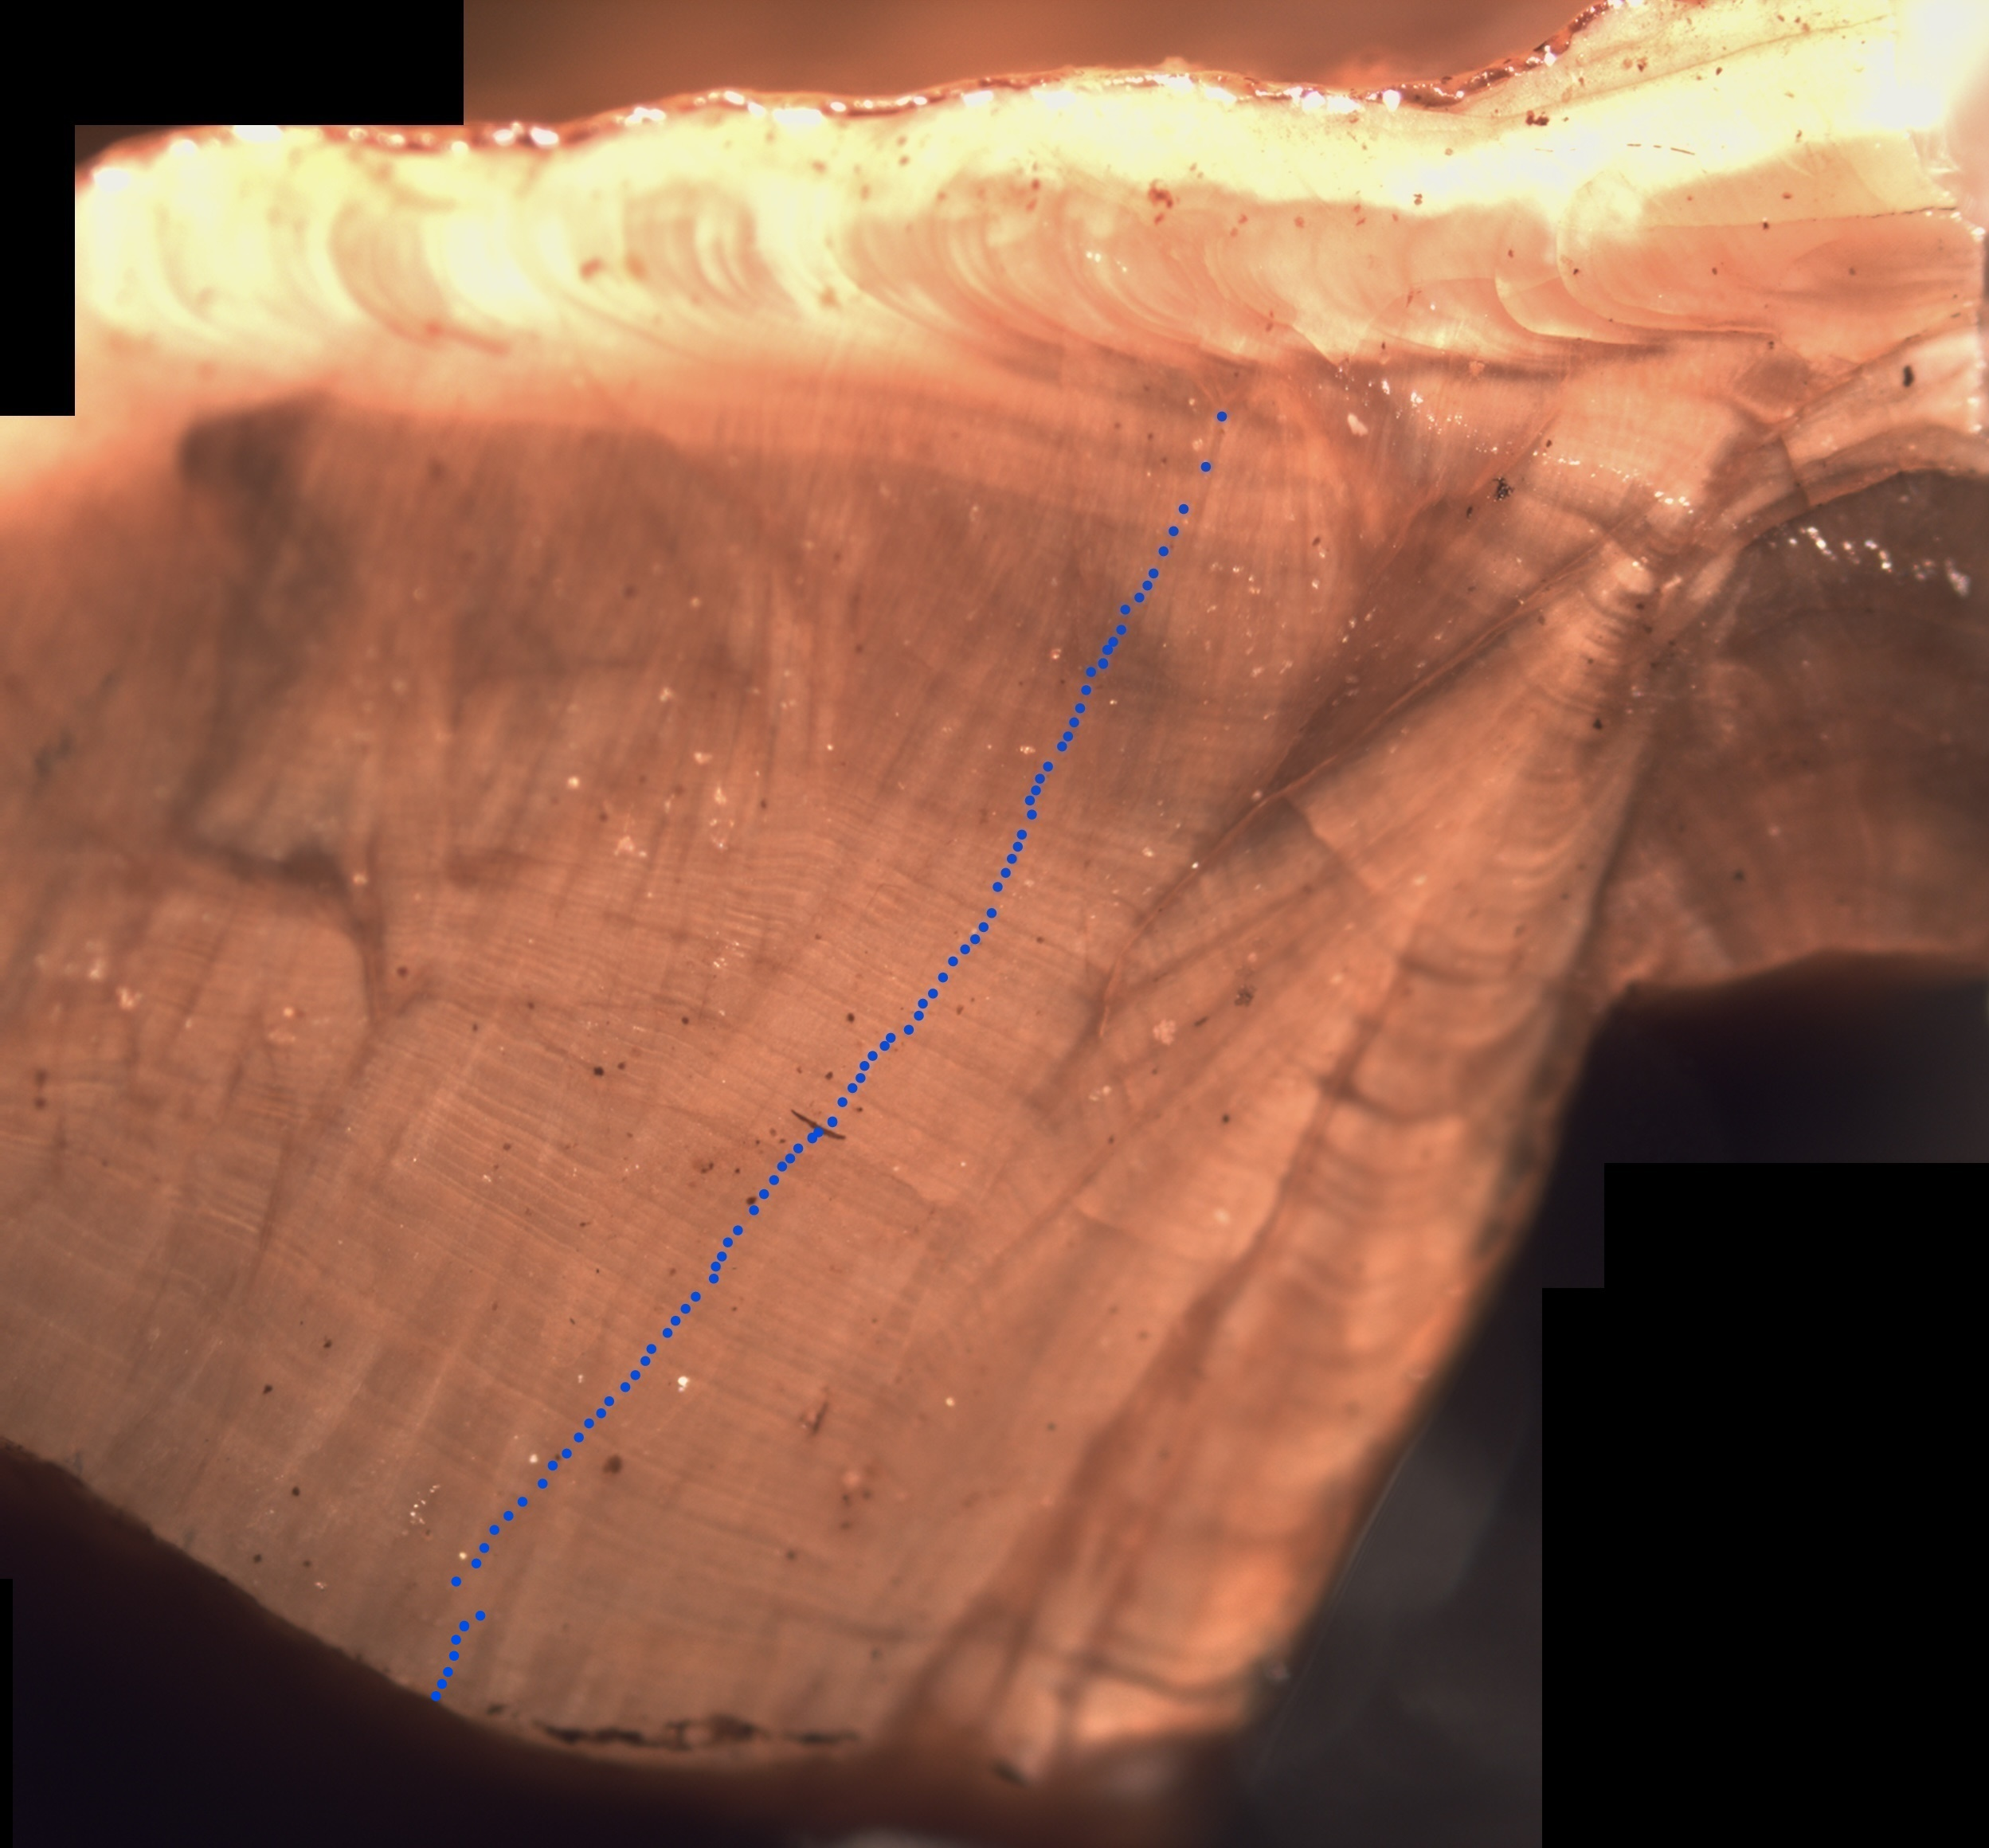
\includegraphics[width=1\textwidth,height=1\textheight]{C:/Stock_Assessments/VRML_Assessment_2021/GitHub/Vermilion_2021/doc/figures/oldfish.jpg}
\caption{Photograph of the \emph{oldest} aged fish used in the assessment with annuli marked by B. Kamikawa (NWFSC)..\label{fig:fig-oldfish}}
\end{figure}

\begin{figure}
\centering
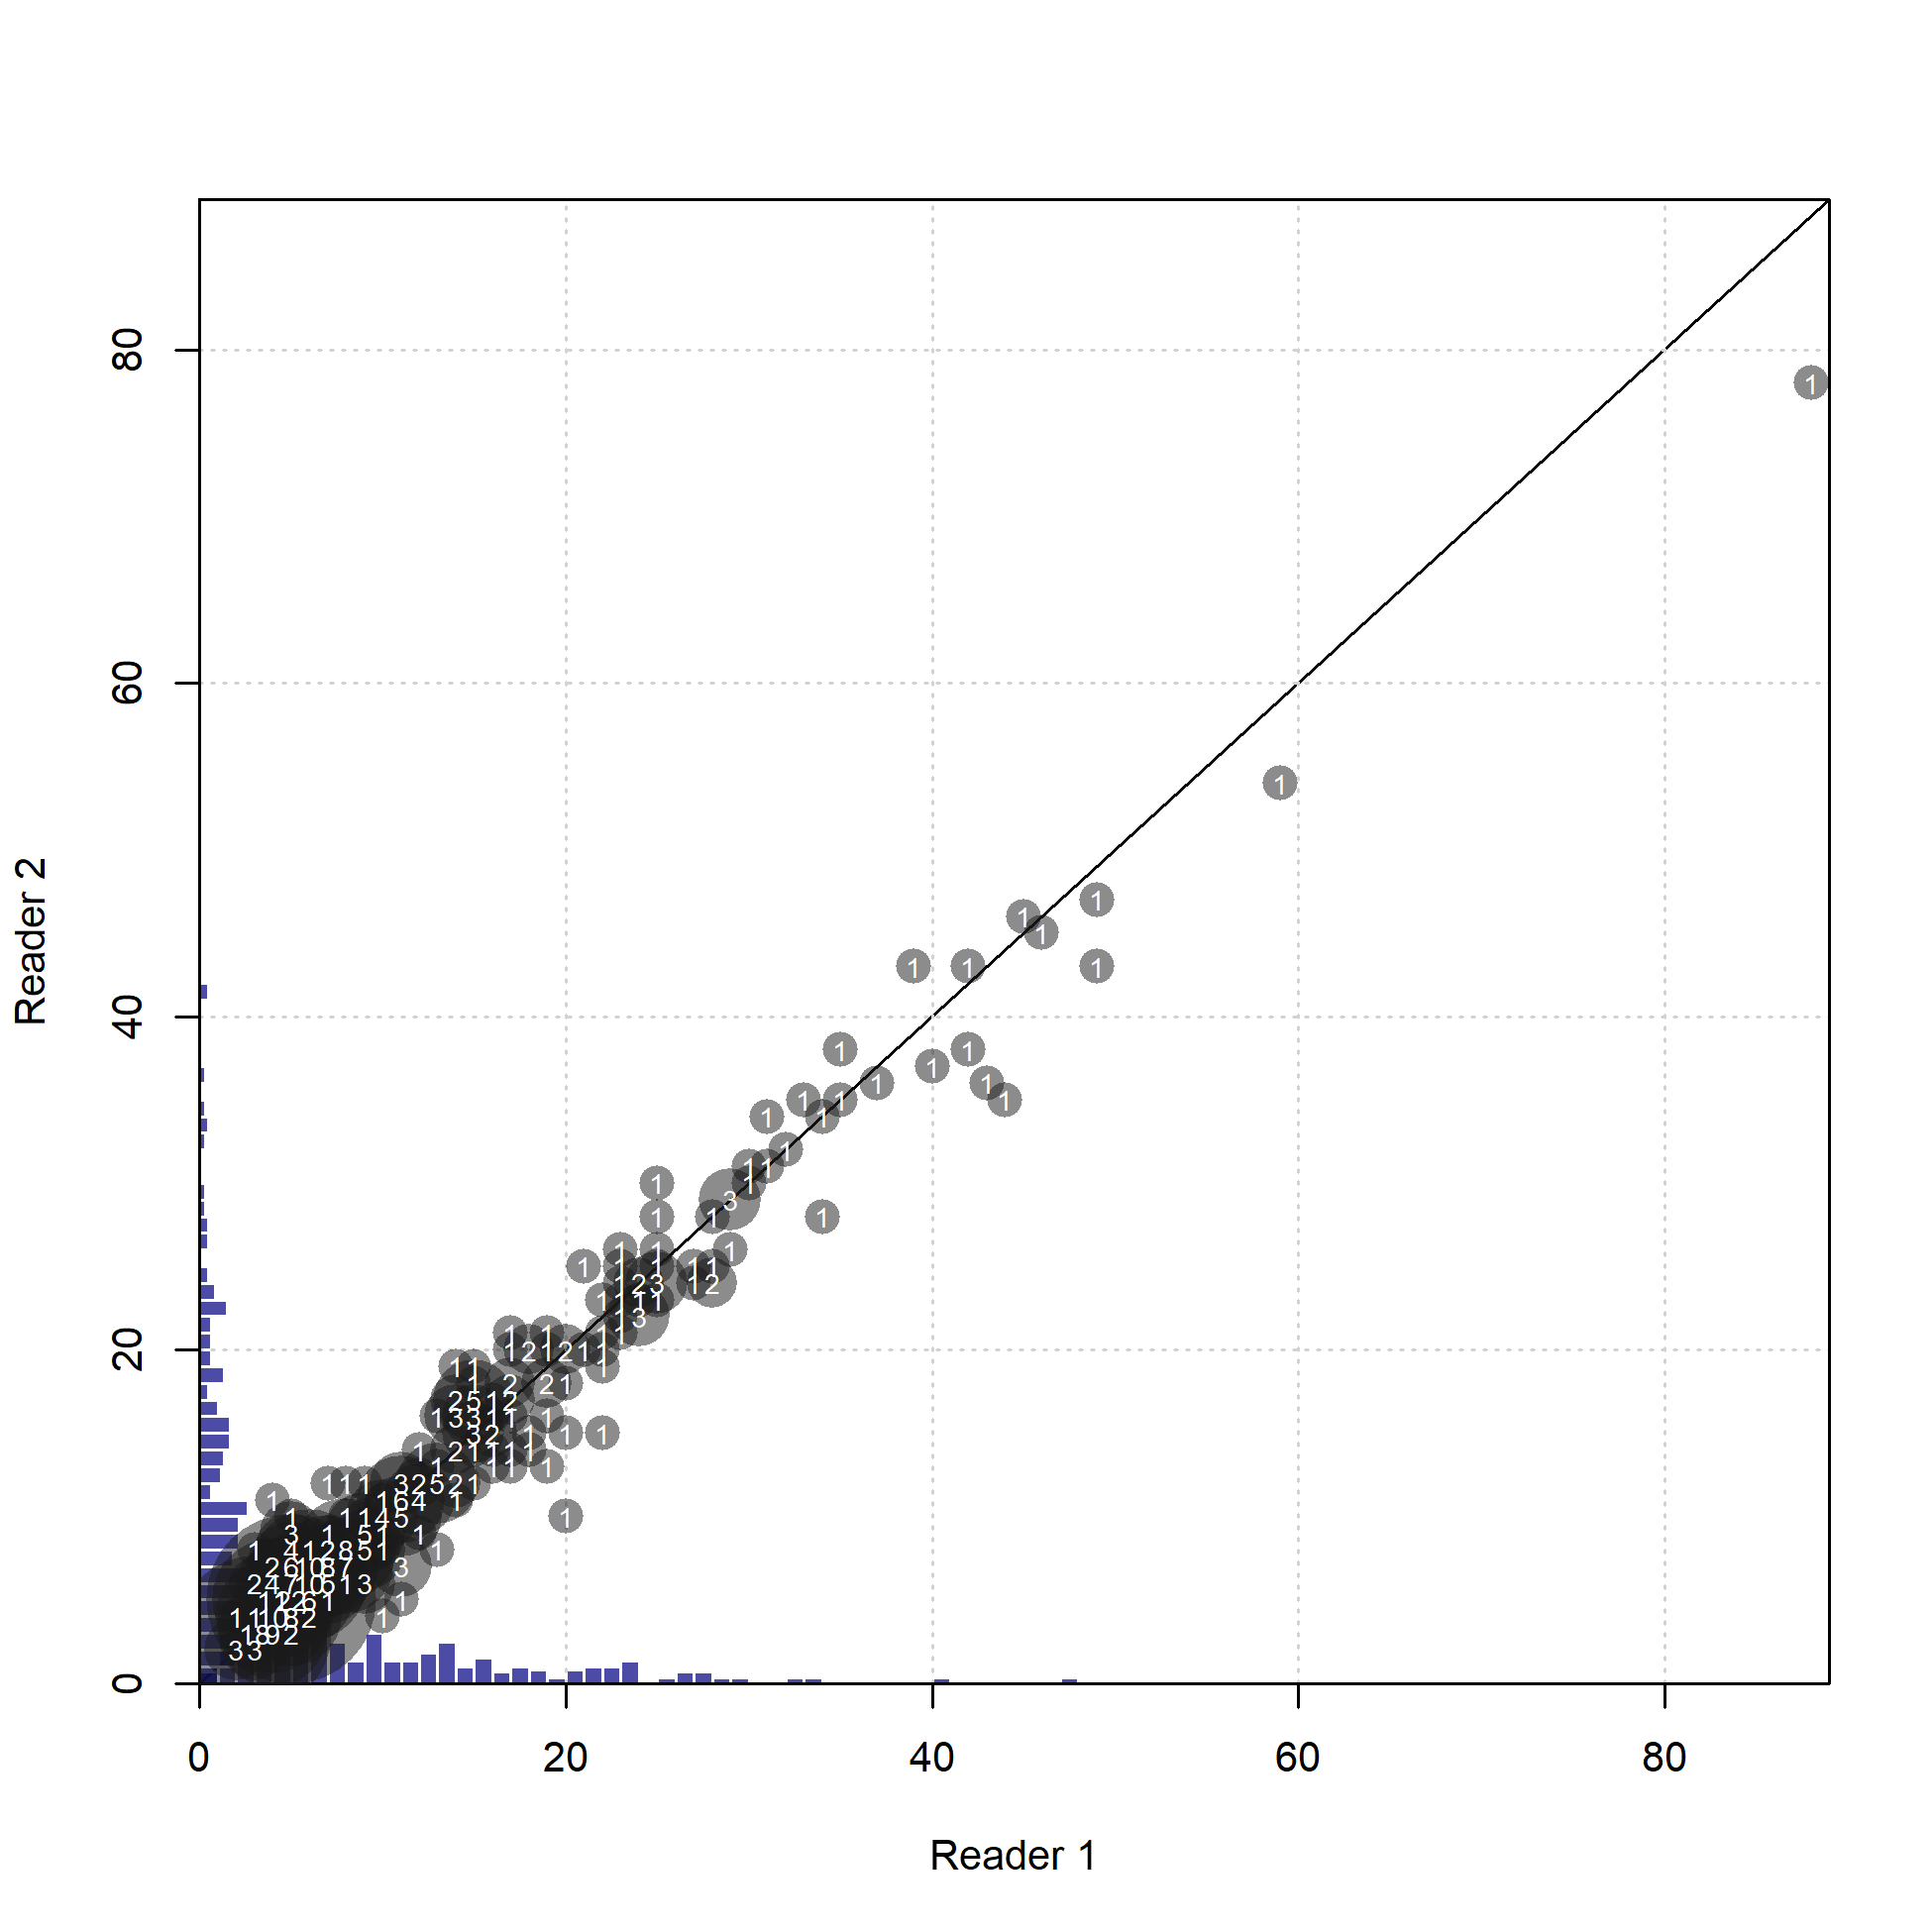
\includegraphics[width=1\textwidth,height=1\textheight]{C:/Stock_Assessments/VRML_Assessment_2021/GitHub/Vermilion_2021/doc/figures/Reader 1 vs Reader 2.png}
\caption{Aging precision between initial and blind double reads for vermilion. Numbers in the bubbles are the sample sizes of otoliths cross-read..\label{fig:fig-reader1reader2}}
\end{figure}

\begin{figure}
\centering
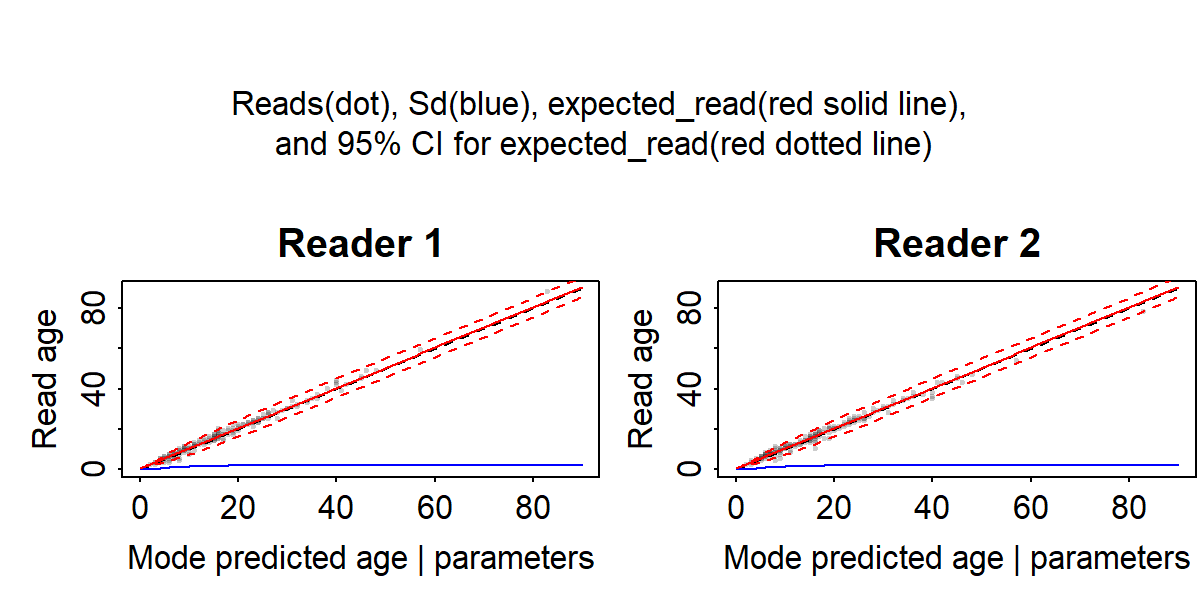
\includegraphics[width=1\textwidth,height=1\textheight]{C:/Stock_Assessments/VRML_Assessment_2021/GitHub/Vermilion_2021/doc/figures/True vs Reads (by reader).png}
\caption{True versus predicted age for two current age readers at the NWFSC from the ageing error software with unbiased reads for reader 1 and curvilinear bias for reader 1 and curvilinear standard deviation for both readers..\label{fig:fig-truereads}}
\end{figure}

\begin{figure}
\centering
\includegraphics[width=1\textwidth,height=1\textheight]{C:/Stock_Assessments/VRML_Assessment_2021/Model_files/NCA/Verm21NoCA_060_time-varying_PC_and_PR/plots/sel01_multiple_fleets_length1.png}
\caption{Selectivity at length by fleet.\label{fig:fig-selex}}
\end{figure}

\begin{figure}
\centering
\includegraphics[width=1\textwidth,height=1\textheight]{C:/Stock_Assessments/VRML_Assessment_2021/Model_files/NCA/Verm21NoCA_060_time-varying_PC_and_PR/plots/SPR2_minusSPRseries.png}
\caption{Estimated 1 - relative spawning ratio (SPR) by year.\label{fig:fig-1-spr}}
\end{figure}

\newpage

\clearpage

\tagstructbegin{tag=H1}\tagmcbegin{tag=H1}

\hypertarget{appendix}{%
\section{Appendix}\label{appendix}}

\leavevmode\tagmcend\tagstructend

\tagstructbegin{tag=H2}\tagmcbegin{tag=H2}

\hypertarget{debwv}{%
\subsection{Deb Wilson-Vandenberg Index of Abundance}\label{debwv}}

\leavevmode\tagmcend\tagstructend

\tagstructbegin{tag=H3}\tagmcbegin{tag=H3}

\hypertarget{deb-wilson-vandenberg-index}{%
\subsubsection{Deb Wilson-Vandenberg Index}\label{deb-wilson-vandenberg-index}}

\leavevmode\tagmcend\tagstructend

The Deb Wilson-Vanedenberg data set is an onboard observer survey data conducted by CDFW survey in central California from 1987-1998 and referred to as the Deb Wilson-Vandenberg onboard observer survey, {\tagstructbegin{tag=Reference}\tagmcbegin{tag=Reference}(\textbf{Reilly1998?})\leavevmode\tagmcend\tagstructend}). During an onboard observer trip the sampler rides along on the CPFV and records location-specific catch and discard information to the species level for a subset of anglers onboard the vessel. The subset of observed anglers is usually a maximum of 15 people the observed anglers change during each fishing stop. The catch cannot be linked to an individual, but rather to a specific fishing location. The sampler also records the starting and ending time, number of anglers observed, starting and ending depth, and measures discarded fish. The fine-scale catch and effort data allow us to better filter the data for indices to fishing stops within suitable habitat for the target species.

\textbf{Deb Wilson-Vandenberg Index: Data Preparation, Filtering, and Sample Sizes}

A large effort was made by the SWFSC to recover data from the original data sheets for this survey and developed into a relational database {\tagstructbegin{tag=Reference}\tagmcbegin{tag=Reference}(\textbf{Monk2016?})\leavevmode\tagmcend\tagstructend}. The specific fishing locations at each fishing stop were recorded at a finer scale than the catch data for this survey. We aggregated the relevant location information (time and number of observed anglers) to match the available catch information. Between April 1987 and July 1992 the number of observed anglers was not recorded for each fishing stop, but the number of anglers aboard the vessel is available. We imputed the number of observed anglers using the number of anglers aboard the vessel and the number of observed anglers at each fishing stop from the August 1992-December 1998 data (see Supplemental materials for details). In 1987, trips were only observed in Monterey, CA and were therefore excluded from the analysis (Table \ref{tab:tab-data-filter-debwv}). Sampling targeted areas of central California. Of the 2,256 trips observed, only 12 of those launched from port in District 6, which was removed from the analysis.

Each fishing location was assigned to a reef based on the on the bathymetric maps and interpretation o hard bottom was extracted from the {\tagstructbegin{tag=Link}\tagmcbegin{tag=Link}\href{http://seafloor.otterlabs.org/index.html}{California Seafloor Mapping Project}\leavevmode\tagmcend\tagstructend}. Reefs were aggregated to four regions produce adequate sample sizes; Ft. Bragg to Santa Cruz (V1), Moss Landing to Big Sur (V2), San Luis Obispo to Pt. Conception (V3)", and Offshore (deeper) locations including the Farallon Islands and reefs of Half Moon Bay and Monterey Bay (V4). The ports in San Luis Obispo county were sampled more frequently than other regions and CPUE is also higher in this area (Figure \ref{fig:fig-areacpue-debwv})

We retained 6597 drifts for index standardization, with 2016 fishing location encountering vermilion.\\
Tables of the number of samples and positive observervations by factor can be found in Tables (\ref{tab:tab-depth-debwv}, \ref{tab:tab-region-debwv}, and \ref{tab:tab-year-debwv}).

\textbf{Deb Wilson-Vandenberg Index: Model Selection, Fits, and Diagnostics}

AA Gamma model was selected for the positive observation GLM by a {\tagstructbegin{tag=Formula}\tagmcbegin{tag=Formula}\(\Delta AIC\)\leavevmode\tagmcend\tagstructend} of 5529.18 over a Lognormal model. The delta-GLM method allows the linear predictors to differ between the binomial and positive models. Based on AIC values from maximum likelihood fits Table \ref{tab:tab-model-select-debwv}), a main effects model including YEAR and MegaReef and WAVE and DEPTH\_bin was fit for the binomial model and a main effects model including YEAR and MegaReef and WAVE and DEPTH\_bin was fit for the Gamma model. Models were fit using the ``rstanarm'' R package (version 2.21.1). Posterior predictive checks of the Bayesian model fit for the binomial model and the positive model were all reasonable (Figures \ref{fig:fig-posterior-mean-debwv} and \ref{fig:fig-posterior-sd-debwv}). The binomial model generated data sets with the proportion zeros similar to the 69\% zeroes in the observed data (Figure \ref{fig:fig-propzero-debwv}). The predicted marginal effects from both the binomial and Gamma models can be found in (Figures \ref{fig:fig-Dbin-marginal-debwv} and \ref{fig:fig-Dpos-marginal-debwv}). The final index (Table \ref{tab:tab-index-debwv}) represents a similar trend to the arithmetic mean of the annual CPUE (Figure \ref{fig:fig-cpue-debwv}).

\begin{table}

\caption{\label{tab:tab-data-filter-debwv}Data filtering steps DebWV onboard survey index for vermilion in NCA .}
\centering
\begin{tabular}[t]{llrrl}
\toprule
Filter & Desciption & Drift & Positive Drifts & Percent drifts retained\\
\midrule
\cellcolor{gray!6}{All} & \cellcolor{gray!6}{None} & \cellcolor{gray!6}{7566} & \cellcolor{gray!6}{2593} & \cellcolor{gray!6}{34\%}\\
No catch & Remove no catch trips & 7041 & 2068 & 29\%\\
\cellcolor{gray!6}{Sparse data} & \cellcolor{gray!6}{Remove District 6 and 1987} & \cellcolor{gray!6}{6697} & \cellcolor{gray!6}{2022} & \cellcolor{gray!6}{30\%}\\
Time fished & Remove drifts fished less than 6 minutes & 6597 & 2016 & 31\%\\
\bottomrule
\end{tabular}
\end{table}

\begin{table}

\caption{\label{tab:tab-depth-debwv}Positive samples of vermilion in NCA by depth (fm).}
\centering
\begin{tabular}[t]{lrrl}
\toprule
Depth & Drifts & Positive Drifts &  Percent Positive Drifts\\
\midrule
\cellcolor{gray!6}{(0,10]} & \cellcolor{gray!6}{478} & \cellcolor{gray!6}{113} & \cellcolor{gray!6}{24\%}\\
(10,20] & 1344 & 455 & 34\%\\
\cellcolor{gray!6}{(20,30]} & \cellcolor{gray!6}{1198} & \cellcolor{gray!6}{410} & \cellcolor{gray!6}{34\%}\\
(30,40] & 1331 & 465 & 35\%\\
\cellcolor{gray!6}{(40,50]} & \cellcolor{gray!6}{1067} & \cellcolor{gray!6}{347} & \cellcolor{gray!6}{33\%}\\
\addlinespace
(50,60] & 617 & 172 & 28\%\\
\cellcolor{gray!6}{(60,70]} & \cellcolor{gray!6}{263} & \cellcolor{gray!6}{36} & \cellcolor{gray!6}{14\%}\\
(70,118] & 299 & 18 & 6\%\\
\bottomrule
\end{tabular}
\end{table}

\begin{table}

\caption{\label{tab:tab-region-debwv}Positive samples of vermilion in NCA by subregion used in the index.}
\centering
\begin{tabular}[t]{lrrl}
\toprule
Region & Drifts & Positive Drifts & Percent Positive Drifts\\
\midrule
\cellcolor{gray!6}{Ft. Bragg to Santa Cruz (V1)} & \cellcolor{gray!6}{1317} & \cellcolor{gray!6}{362} & \cellcolor{gray!6}{27\%}\\
Moss Landing to Big Sur (V2) & 1448 & 322 & 22\%\\
\cellcolor{gray!6}{San Luis Obispo to Pt. Conception (V3)} & \cellcolor{gray!6}{1668} & \cellcolor{gray!6}{924} & \cellcolor{gray!6}{55\%}\\
Offshore (V4) & 2164 & 408 & 19\%\\
\bottomrule
\end{tabular}
\end{table}

\begin{table}

\caption{\label{tab:tab-year-debwv}Samples by year of vermilion in NCA from the  DebWVCPFV survey by depth (fm).}
\centering
\begin{tabular}[t]{lrrl}
\toprule
Year & Drifts & Positive drifts & Percent Positive Drifts\\
\midrule
\cellcolor{gray!6}{1988} & \cellcolor{gray!6}{422} & \cellcolor{gray!6}{136} & \cellcolor{gray!6}{32\%}\\
1989 & 446 & 170 & 38\%\\
\cellcolor{gray!6}{1990} & \cellcolor{gray!6}{122} & \cellcolor{gray!6}{65} & \cellcolor{gray!6}{53\%}\\
1991 & 135 & 73 & 54\%\\
\cellcolor{gray!6}{1992} & \cellcolor{gray!6}{467} & \cellcolor{gray!6}{168} & \cellcolor{gray!6}{36\%}\\
\addlinespace
1993 & 485 & 196 & 40\%\\
\cellcolor{gray!6}{1994} & \cellcolor{gray!6}{555} & \cellcolor{gray!6}{189} & \cellcolor{gray!6}{34\%}\\
1995 & 791 & 247 & 31\%\\
\cellcolor{gray!6}{1996} & \cellcolor{gray!6}{963} & \cellcolor{gray!6}{238} & \cellcolor{gray!6}{25\%}\\
1997 & 1312 & 323 & 25\%\\
\addlinespace
\cellcolor{gray!6}{1998} & \cellcolor{gray!6}{899} & \cellcolor{gray!6}{211} & \cellcolor{gray!6}{23\%}\\
\bottomrule
\end{tabular}
\end{table}

\begin{table}

\caption{\label{tab:tab-model-select-debwv}Model selection for the DebWV onboard survey index for vermilion in NCA .}
\centering
\begin{tabular}[t]{lrr}
\toprule
Model & Binomial $\Delta$AIC & Gamma $\Delta$AIC\\
\midrule
\cellcolor{gray!6}{1} & \cellcolor{gray!6}{1011.38} & \cellcolor{gray!6}{402.07}\\
YEAR + MegaReef & 169.08 & 80.84\\
\cellcolor{gray!6}{YEAR + MegaReef + WAVE} & \cellcolor{gray!6}{120.32} & \cellcolor{gray!6}{57.19}\\
YEAR + MegaReef + WAVE + DEPTH bin & 0.00 & 0.00\\
\cellcolor{gray!6}{YEAR + WAVE + DEPTH bin} & \cellcolor{gray!6}{611.73} & \cellcolor{gray!6}{252.61}\\
\addlinespace
YEAR + DEPTH bin & 642.50 & 402.07\\
\cellcolor{gray!6}{YEAR + MegaReef + DEPTH bin} & \cellcolor{gray!6}{55.30} & \cellcolor{gray!6}{14.94}\\
\bottomrule
\end{tabular}
\end{table}

\begin{table}

\caption{\label{tab:tab-index-debwv}Standardized index for the DebWVCPFV survey index with log-scale standard errors and 95% highest 
       posterior density (HPD) intervals for vermilion in NCA .}
\centering
\begin{tabular}[t]{rrrrr}
\toprule
Year & Mean & logSE & lower HPD & upper HPD\\
\midrule
\cellcolor{gray!6}{1988} & \cellcolor{gray!6}{0.03} & \cellcolor{gray!6}{0.22} & \cellcolor{gray!6}{0.02} & \cellcolor{gray!6}{0.05}\\
1989 & 0.04 & 0.20 & 0.03 & 0.06\\
\cellcolor{gray!6}{1990} & \cellcolor{gray!6}{0.09} & \cellcolor{gray!6}{0.23} & \cellcolor{gray!6}{0.06} & \cellcolor{gray!6}{0.14}\\
1991 & 0.04 & 0.24 & 0.03 & 0.07\\
\cellcolor{gray!6}{1992} & \cellcolor{gray!6}{0.04} & \cellcolor{gray!6}{0.20} & \cellcolor{gray!6}{0.03} & \cellcolor{gray!6}{0.06}\\
\addlinespace
1993 & 0.04 & 0.20 & 0.03 & 0.05\\
\cellcolor{gray!6}{1994} & \cellcolor{gray!6}{0.03} & \cellcolor{gray!6}{0.20} & \cellcolor{gray!6}{0.02} & \cellcolor{gray!6}{0.05}\\
1995 & 0.03 & 0.20 & 0.02 & 0.04\\
\cellcolor{gray!6}{1996} & \cellcolor{gray!6}{0.02} & \cellcolor{gray!6}{0.21} & \cellcolor{gray!6}{0.01} & \cellcolor{gray!6}{0.03}\\
1997 & 0.03 & 0.19 & 0.02 & 0.04\\
\addlinespace
\cellcolor{gray!6}{1998} & \cellcolor{gray!6}{0.03} & \cellcolor{gray!6}{0.21} & \cellcolor{gray!6}{0.02} & \cellcolor{gray!6}{0.05}\\
\bottomrule
\end{tabular}
\end{table}

\FloatBarrier

\begin{figure}
\centering
\includegraphics{C:/Stock_Assessments/VRML_Assessment_2021/GitHub/Vermilion_2021/doc/indices/vermilion_DebWV_onboard_writeup_NCA_files/figure-latex/fig-areacpue-debwv-1.pdf}
\caption{\label{fig:fig-areacpue-debwv}Arithmetic mean of CPUE by region for vermilion from the filtered data. Definitions of areas used are in the text.}
\end{figure}

\begin{figure}
\centering
\includegraphics{C:/Stock_Assessments/VRML_Assessment_2021/GitHub/Vermilion_2021/doc/indices/vermilion_DebWV_onboard_writeup_NCA_files/figure-latex/fig-cpue-debwv-1.pdf}
\caption{\label{fig:fig-cpue-debwv}Standardized index and arithmetic mean of the CPUE from the filtered data. Each timeseries is scaled to its respective means.}
\end{figure}

\begin{figure}
\centering
\includegraphics{C:/Stock_Assessments/VRML_Assessment_2021/GitHub/Vermilion_2021/doc/indices/vermilion_DebWV_onboard_writeup_NCA_files/figure-latex/fig-propzero-debwv-1.pdf}
\caption{\label{fig:fig-propzero-debwv}Posterior predictive distribution of the proportion of zero observations in replicate data sets generated by the delta model with a vertical line representing the observed average.}
\end{figure}

\begin{figure}
\centering
\includegraphics{C:/Stock_Assessments/VRML_Assessment_2021/GitHub/Vermilion_2021/doc/indices/vermilion_DebWV_onboard_writeup_NCA_files/figure-latex/fig-posterior-mean-debwv-1.pdf}
\caption{\label{fig:fig-posterior-mean-debwv}Posterior predictive draws of the mean by year with a vertical line of the raw data average.}
\end{figure}

\begin{figure}
\centering
\includegraphics{C:/Stock_Assessments/VRML_Assessment_2021/GitHub/Vermilion_2021/doc/indices/vermilion_DebWV_onboard_writeup_NCA_files/figure-latex/fig-posterior-sd-debwv-1.pdf}
\caption{\label{fig:fig-posterior-sd-debwv}Posterior predictive draws of the standard deviation by year with a vertical line of the raw average}
\end{figure}

\begin{figure}
\centering
\includegraphics{C:/Stock_Assessments/VRML_Assessment_2021/GitHub/Vermilion_2021/doc/indices/vermilion_DebWV_onboard_writeup_NCA_files/figure-latex/fig-Dbin-marginal-debwv-1.pdf}
\caption{\label{fig:fig-Dbin-marginal-debwv}Binomial marginal effects from the final model}
\end{figure}

\begin{figure}
\centering
\includegraphics{C:/Stock_Assessments/VRML_Assessment_2021/GitHub/Vermilion_2021/doc/indices/vermilion_DebWV_onboard_writeup_NCA_files/figure-latex/fig-Dpos-marginal-debwv-1.pdf}
\caption{\label{fig:fig-Dpos-marginal-debwv}Positive model marginal effects from the final model.}
\end{figure}

\hypertarget{refs}{}
\begin{CSLReferences}{1}{0}
\leavevmode\vadjust pre{\hypertarget{ref-Hamel2015}{}}%
Hamel, Owen S. 2015. {``{A method for calculating a meta-analytical prior for the natural mortality rate using multiple life history correlates}.''} \emph{ICES Journal of Marine Science} 72 (1): 62--69. \url{https://doi.org/doi:10.1093/icesjms/fsu131}.

\leavevmode\vadjust pre{\hypertarget{ref-Then2018}{}}%
Then, Amy Y., John M. Hoenig, Norman G. Hall, and David A. Hewitt. 2018. {``{Evaluating the predictive performance of empirical estimators of natural mortality rate using information on over 200 fish species}.''} \emph{ICES Journal of Marine Science} 75 (4): 1509. \url{https://doi.org/10.1093/icesjms/fsx199}.

\leavevmode\vadjust pre{\hypertarget{ref-Thorson2012}{}}%
Thorson, James T., Ian J. Stewart, and André E. Punt. 2012. {``{Development and application of an agent-based model to evaluate methods for estimating relative abundance indices for shoaling fish such as Pacific rockfish (\emph{Sebastes} spp.)}.''} \emph{ICES Journal of Marine Science} 69 (4): 635--47.

\end{CSLReferences}
\end{document}
